
\section{Ultrasound Design Gallery}\label{section:usdg}

%In this section, we introduce the~\textsc{Ultrasound Design Gallery} (USDG).
%The USDG is primarily based on two components: a user interface (\cref{section:ui}) and an algorithm for learning (\cref{section:gp}) and optimizing the sonographer's subjective image quality metric (\cref{section:bo}).

\subsection{Problem Statement}
Let us denote a setting (or parameters) of an image enhancement algorithm as \(\vx \in \mathcal{X}\).
Given a specific clinical task \(t\), we assume an individual sonographer \(s\) has a subjective image quality function \(f\), which is possibly noisy.
For a setting \(\vx\), the sonographer rates the images processed by the algorithm as \(f\left(\vx\right)\).
Our goal is to solve the problem
%
\begin{align*}
  \maximize_{\vx \in \mathcal{X}} \mathbb{E}\left[\,f\left(\vx; t, s \right)\,\right]
\end{align*}
%
and find the optimal setting \(\vx^*\) that maximizes \(f\).

Naturally, we do not have access to the subjective image quality function \(f\).
Instead, we query the sonographer to provide preferential feedback (\cref{section:ui}), which we use to probabilistically infer \(f\) (\cref{section:gp}).
Using this knowledge, we progressively design new queries so that we can eventually find the optimal setting \(\vx^*\) (\cref{section:bo}).

\subsection{User Interface of the Ultrasound Design Gallery}\label{section:ui}
\subsubsection{Preferential Feedback with Design Galleries}
Humans are notoriously bad at quantifying their absolute preferences.
However, when asked to \textit{compare} different choices, they are more capable at telling which one they prefer over the others~\cite{10.2307/27821441, NIPS2007_b6a1085a}.
The \textit{Design Gallery}~\cite{10.1145/258734.258887} interface builds upon this principle.
It optimizes human preference by displaying multiple choices to the user and letting him choose which one he/she prefers over the others.

The original Design Gallery by Marks \textit{et al.}~\cite{10.1145/258734.258887} and its variant by Brochu et al.~\cite{brochu_bayesian_2010} propose a discrete set of choices \(A = \{\vx_1, \vx_2,{\,\ldots\,}, \vx_N\}\) to the user.
Each time the user chooses an optimal choice \(\vx^*\), we obtain the preferential feedback that \(\vx^* \succ \vx_i,\; \forall\vx_i \in A \setminus \vx^* \) where \(\succ\) denotes preferential ordering.
Naturally, proposing a large number of candidates increases the informativeness of a single user choice.
By extrapolating this intuition, Koyama \textit{et al.}~proposed design galleries that suggest a continuous set of choices embedded on a 1D line~\cite{10.1145/3072959.3073598} and a 2D plane~\cite{koyama_sequential_2020}.

Medical ultrasound images are best presented in a sequence of images rather than still images.
In this case, embedding multiple videos on a 2D plane can be visually confusing, which is why we base our USDG on the 1D sequential line search scheme proposed by Koyama \textit{et al.}~\cite{10.1145/3072959.3073598}.

\subsubsection{Overview of the Ultrasound Design Gallery Interface}
%
\begin{figure}[t]
  \vspace{-0.2in}
  \centering
  \includegraphics[scale=0.30]{figures/ui.png}
  \caption{User interface of the Ultrasound Design Gallery. The \textbf{video (preview) window} (left), the \textbf{line search window} (top right), and the \textbf{video control window} (bottom right) are shown.}\label{fig:ui}
  \vspace{-0.1in}
\end{figure}
%
The user interface of the USDG is shown in~\cref{fig:ui}.
It comprises of three basic components:
    %\vspace{0.05in}
\begin{enumerate}
  \item[\ding{228}] \textbf{Video (preview) window}: This window displays the image processed using the currently chosen setting.
    %\vspace{0.05in}
  \item[\ding{228}] \textbf{Line search window}: This window contains the 1D slider on which the proposed settings are embedded.
    %\vspace{0.05in}
  \item[\ding{228}] \textbf{Video control window}: This window provides basic controls over the image presentation such as dynamic range and frame rate.
\end{enumerate}
The sonographer compares different settings by interacting with the slider on the~\textbf{line search window}.
Each position of the slider represents a different setting which is embedded on the 1D line.
The \textbf{video window} presents a pre-recorded sequence of ultrasound images processed with the chosen setting in real-time.
This process is illustrated in~\cref{fig:interaction}

\subsubsection{Interacting with the Ultrasound Design Gallery}
%
\begin{figure}[t]
  \vspace{-0.2in}
  \centering
  \includegraphics[scale=0.27]{figures/ui_interaction.pdf}
  \caption{Visualization of the interaction with the USDG}\label{fig:interaction}
  \vspace{-0.15in}
\end{figure}
%
The basic workflow of using the USDG is as follows:
\begin{enumerate}
\item[\ding{182}] The sonographer is first presented with images processed using randomly sampled settings.
\item[\ding{183}] The sonographer compares the random settings embedded on the 1D line by interacting with the slider and approves the setting he/she preferred the most. This process is illustrated in~\cref{fig:interaction}.
\item[\ding{184}] The USDG records the choice and infers the subjective quality metric \(f\) of the sonographer (\textbf{\cref{section:gp}}).
\item[\ding{185}] Based on the inferred model, the USDG recommends a new set of settings embedded on the 1D slider through Bayesian optimization (\textbf{\cref{section:bo}}).
\item[\ding{186}] The sonographer compares the new settings by interacting with the slider as in step~\ding{183}.
\item[\ding{187}] Go back to step~\ding{184} until convergence.
\end{enumerate}

\begin{figure}[t]
  \centering
  \includegraphics[scale=0.35]{figures/linesearch.pdf}
  \caption{Visualization of the relationship between the slider interface and the parameter space \(\mathcal{X}\).
    We show a two-dimensional parameter space \(\mathcal{X} = {[0, 1]}^2\) for illustration.
    The 1D embedding is formed by the basis vector \(\vx\) and the direction vector \(\vxi\).
  }\label{fig:linesearch}
  \vspace{-0.15in}
\end{figure}
%
Formally, at each BO iteration \(t\), the user conceptually solves the line search problem
\begin{align}
 \alpha_t = &\argmax_{ \beta }\; f\,(\beta\,\vxi_t + \vx_t) \label{eq:line_search}\\
 &\text{subject to}\;\; \beta \in \mathcal{I}\left(\vx_t, \vxi_t\right) \nonumber
\end{align}
{\noindent}where \(\beta\) is a position on the 1D line, \(\vx_t\) and \(\vxi_t\) are the basis and direction of the 1D line, \(\mathcal{X}\) is the domain of all the parameter settings, and \(\mathcal{I}\left(\vx_t, \vxi_t\right)\) is the set of \(\beta\)s that satisfy \(\beta\,\vxi + \vx  \in \mathcal{X}\).
The choice maximizing \(f\) is denoted as \(\alpha_t\).
The correspondence between the graphical interface and our mathematical notations is visualized in~\cref{fig:linesearch}.
After the user successively solves this line search problem, the USDG gradually converges towards the best parameter setting \(\vx^{*}\).

\subsection{Learning the Preference of Sonographers}\label{section:gp}
\subsubsection{Probabilistic Model}
%\paragraph{Gaussian Process Formulation}
We infer the subjective quality metric \(f\) using probabilistic machine learning given the preferential feedback.
We take a Bayesian learning approach.
At the \(t\)th iteration, a single preferential feedback is fully represented by \((\alpha_t, \vx_t, \vxi_t)\) since the 1D line is formed by \(\vx_t, \vxi_t\), and the optimal position on the line is given by \(\alpha_t\).
The history of preferential feedback from iteration 1 to \(T\) forms a dataset
%
\begin{align*}
  \mathcal{D}_T = \{\,(\vx_1, \vxi_1, \alpha_1),\, \ldots\,, (\vx_t, \vxi_t, \alpha_t),\,\ldots\,, (\vx_T, \vxi_T, \alpha_T) \,\}
\end{align*}
%
where the ordering
\begin{align*}
f(\alpha_t\,\vx_t + \vxi_t ) > f(\beta^{(i)}\,\vx_t + \vxi_t) \;\;\text{for all}\;\; \beta^{(i)} \in \mathcal{I}\left(\vx, \vxi\right) \setminus \alpha_t
\end{align*}
is satisfied.
Each datapoint forms an infinite number of orderings since \(\mathcal{I}\left(\vx, \vxi\right)\) contains an infinite number of \(\beta\)s.

We perform Bayesian inference of the latent preference function \(f\) by setting a Gaussian process prior~\cite{rasmussen_gaussian_2006}.
Our probabilistic model is stated as 
%
{
\begin{align*}
\ell          \;&\sim \; p\,(\ell) \\
\epsilon_{\vf} \;&\sim \; p\,(\epsilon_{\vf}) \\
\sigma        \;&\sim \; p\,(\sigma) \\
\vf           \;&\sim \; \mathcal{GP}(0, \mK_{\ell} + \epsilon_{\vf}^2\mI) \\
\begin{matrix}
\; f(\alpha_t\,\vxi + \vx_t) > f(\beta\,\vxi_t + \vx_t), \; \\
\; \forall\beta \in \mathcal{I}\left(\vx_t, \vxi_t\right) \setminus \alpha \;
\end{matrix}\; &\sim \; p\left(\cdot \mid\, \vf,\, \sigma,\, \alpha_t,\, \vx_t,\, \vxi_t\,\right) 
\end{align*}
}
{\noindent}where \(\epsilon_{\vf}\) is the noise of the preference evaluations, \(\sigma\) is the noice scale of the comparisons (more details in the next section), \(\vf\) is a vector of the latent function values, and \(\mathcal{\mK}_{\ell}\) is the Gram matrix.
Each element of the Gram matrix is defined as
\(
  {[\mK_{\ell}]}_{i,j} = k\left(\vx^\prime_i, \vx^\prime_j; \ell \right)
\)
where \(k\left(\cdot, \cdot; \ell \right)\) is an isotropic Matern 5/2 covariance kernel with a line scale of \(\ell\), and \({\vx^\prime}_i, {\vx^\prime}_j\) are the positions formed by all the combinations of the different \(\alpha, \beta^{(i)}, \vxi, \vx\) in \(\mathcal{D}_t\).

\subsubsection{Likelihood}
%The most important component in our model is the likelihood function \(p\left(\alpha \, \vxi + \vx \succ \beta^{(i)} \, \vxi + \vx \mid \sigma, \vf \right)\).
%Since our 1D line \(\mathcal{I}\left(\vx, \vxi\right)\) contains an \textit{infinite} number of duels between each \(\beta\) and \(\alpha\), it is difficult to formulate a proper likelihood function.
When only a discrete set of choices are compared, the Bradley-Terry-Luce (BTL) model~\cite{10.1145/3072959.3073598} can be used.
However, in our case, the infinite number of comparisons \(\alpha\) vs. \(\beta\) complicates the design of a likelihood function.
The original work by Koyama \textit{et al.}~\cite{koyama_sequential_2020} chooses to discretize the 1D line and apply the BTL model.
Unfortunately, the theoretical consistency of this scheme is unclear.
%to the continuous limit.

Instead, Mikkola \textit{et al.}~\cite{pmlr-v119-mikkola20a} proposed a principled approach that does not rely on the BTL model and allows for accurate approximation.
By assuming the noise of the comparisons follows a white Gaussian process, they show that the probability of a single comparison is
\begin{align*}
  &p\left(\alpha \, \vxi + \vx \succ \beta^{(i)} \, \vxi + \vx \mid \sigma, \vf \right) \\
  &= 1 - \left(\Phi * \phi \right)\left( \frac{ f\left(\beta^{(i)} \, \vxi + \vx \right) - f\left(\alpha \, \vxi + \vx \right) }{\sigma} \right)
\end{align*}
{\noindent}where \(\left(\Phi*\phi\right)\left(\cdot\right)\) is the convolution between the cummulative density and probability density of the standard Gaussian. 

At the limit of infinitely many \(\beta\)s, the likelihood of the discrete comparisons converges to a type-I Volterra integral such that
{\small
\begin{align*}
  &p\left(\alpha \vxi + \vx \succ \beta \vxi + \vx,\; \forall \beta \in \mathcal{I}\left(\vx, \vxi\right) \mid\, \vf,\, \sigma,\, \alpha,\, \vx,\, \vxi\,\right)  \\
  &= \lim_{N \rightarrow \infty} \prod^{N}_{i=1} p\left(\alpha \, \vxi + \vx \succ \beta^{(i)} \, \vxi + \vx \mid \sigma,\, \vf \right) \\
  &= \lim_{N \rightarrow \infty} \prod^{N}_{i=1} \left(  1 - \left(\Phi * \phi \right)\left( \frac{ f\left(\beta^{(i)} \, \vxi + \vx \right) - f\left(\alpha \, \vxi + \vx \right) }{\sigma} \right) \right) \\
  &\rightarrow \exp\left(  - \int_{\mathcal{I}\left(\vx, \vxi\right)} \left(\Phi * \phi \right) \left( \frac{ f\left(\beta \, \vxi + \vx \right) - f\left(\alpha \, \vxi + \vx \right) }{\sigma} \right) d\beta \right)
\end{align*}
}%
%
{\noindent}where \(\beta^{(1)}, \ldots, \beta^{(N)}\) is taken to be an increasing sequence partitioning \(\mathcal{I\left(\vx, \vxi\right)}\).

Now, the log-likelihood of the dataset is given as
{\small
\begin{align*}
  &\log p\left(\mathcal{D}_T \mid \sigma,\, \vf \right)  \\
  &= \sum_{t=1}^{T} p\left(\alpha_t \vxi_t + \vx_t \succ \beta \vxi_t + \vx_t,\; \forall \beta \in \mathcal{I}\left(\vx_t, \vxi_t\right) \mid \vf,\, \sigma,\, \alpha_t,\, \vx_t,\, \vxi_t\right) \\
  &= -\sum_{t=1}^{T} \int_{\mathcal{I}\left(\vx_{t}, \vxi_{t}\right)} \left(\Phi * \phi \right) \left( \frac{ f\left(\beta \, \vxi_{t} + \vx_{t} \right) - f\left(\alpha_{t} \, \vxi_{t} + \vx_{t} \right) }{\sigma} \right) d\beta \\
  &\approx -\frac{1}{N}  \sum_{t=1}^{T} \sum_{i=1}^{N_{\beta}} \left(\Phi * \phi \right) \left( \frac{ f\left(\beta^{(i)} \, \vxi_{t} + \vx_{t} \right) - f\left(\alpha_{t} \, \vxi_{t} + \vx_{t} \right) }{\sigma} \right) d\beta
\end{align*}
}%
{\noindent}where the convolution can be accurately approximated with numerical quadrature.
In our case, we use the Gauss-Hermite quadrature with 16 evaluation points.
For the outer integral, Mikkola \textit{et al.} perform Monte Carlo integration by sampling \(\beta^{(1)}, \ldots, \beta^{(N_{\beta})} \) from a truncated generalized normal distribution depending on \(\vx, \vxi\) and \(t\).
This choice is simply heuristic, and they adaptively concentrate \(\beta_i\) towards \(\alpha\) as \(t\) increases.
For the number of Monte Carlo samples, we set \(N_{\beta}=20\).
Considering the Monte Carlo samples, the dataset is now represented as \(\mathcal{D}_{T} = {\{\,(\,\vx_{t},\, \vxi_{t},\, \alpha_{t},\, \beta^{(1)}_{t},\, \ldots\, \beta^{(N_{\beta})}_{t})\,\}}_{t=1}^{T}\).

\subsubsection{Computational Costs}
The maximum memory requirement for storing the dataset is \(\mathcal{O}\left( T^2 \, N_{\beta}^2  \right)\).
Evaluating the likelihood involves a Cholesky decomposition resulting in a time complexity of \(\mathcal{O}\left( T^3 \, N_{\beta}^3 \, N_{\text{quad.}}^3  \right)\) where \(T\) is the maximum number of BO iterations, \(N\) is the number of Monte Carlo samples of \(\beta\), and \(N_{\text{quad.}}\) is the number of quadrature points for the convolution integral.
While the computational complexity might seem expensive, our efficient C++ implementation achieves real-time inference on a laptop.

\begin{figure}[t]
  \vspace{-0.10in}
  \removelatexerror
  \begin{algorithm2e}[H]
    \DontPrintSemicolon
    \SetAlgoLined
    \KwIn{Precomputed Cholesky decomposition of \(\mK\),
      gradient function of the likelihood \(\nabla_{\vf}\, p(\mathcal{D}\mid\vf)\),
      Hessian function of the joint \(\nabla^2_{\vf}\, p(\mathcal{D},\, \vf)\).
    }
    \KwOut{
      \(\vf_{t}\), \(\mW_t\).
    }
    \( \vf_1 \leftarrow \mathbf{0} \)\;
    \Repeat{ until convergence } {
      \(\valpha        \leftarrow \mK\backslash\vf_{t} \)\;
      \(\vg            \leftarrow \nabla_{\vf}\, p(\mathcal{D}\mid\vf)|_{\vf = \vf_t} - \valpha \)\;
      \(\mW_t          \leftarrow -  \nabla^2_{\vf}\, p(\mathcal{D},\, \vf) \)\;
      \(\mB           \leftarrow \mI + \mK \mW \)\;
      \(\mL_{\mB}, \mU_{\mB} \leftarrow \mathrm{lu}\,(\mB) \)\;
      \(\vp           \leftarrow \mL_{\mB} \backslash \mU_{\mB} \backslash \mK \vg \)\;
      \(\vf_{t+1}      \leftarrow \vf_t + \eta \, \vp \)\;
      \(t \leftarrow t + 1\)\;
    }
    \caption{Newton's Method for Laplace's Approximation with Dense Hessians}\label{alg:newton}
  \end{algorithm2e}
  \vspace{-0.20in}
\end{figure}
%
\subsubsection{Inference with Laplace's Approximation}
We approximate the posterior of \(f\), \(p\,(\vf\,|\,\vtheta,\, \mathcal{D})\) where \(\vtheta\) denotes the hyperparameters, with Laplace's approximation~\cite{williams_bayesian_1998}, which involves a second-order Taylor expansion around the maximum of the posterior such that
\begin{align*}
q\,(\vf) = \mathcal{N}\left(\vf;\, \vf^*,\, {(\mK^{-1} + \mW)}^{-1}\right) \approx p\,(\vf \mid \vtheta,\, \mathcal{D})
\end{align*}
where \(\vf^*\) is the maximum a-posteriori estimate such that \(\nabla_{\vf}\, p\,(\vf, \, \vtheta,\, \mathcal{D})|_{\vf = \vf^*} = 0\), \(\mW = -\nabla^2_{\vf}\, p\,(\vf,\,\vtheta,\, \mathcal{D})|_{\vf=\vf^*} \) is the negative Hessian of the likelihood at \(\vf^*\).

In many GP models, the Hessian \(\mH\) often turns out structured.
This allows efficient implementations of Newton's method for finding \(\vf^*\).
For example, Rasmussen and Williams~\cite{rasmussen_gaussian_2006} discuss special cases where \(\mH\) is diagonal or block-diagonal.
Unfortunately, our \(\mH\) is neither.
We thus provide a different implementation of Newton's iteration that assumes \(\mH\) is dense.
Our formulation is based on 
{\small
\begin{align*}
  {\big(\mK^{-1} + \mW\big)}^{-1}
  %&= {\Big(\mK^{-1} \big(\mI + \mK \mW \big)\Big)}^{-1} \\
  \,=\, {{\big(\mI + \mK \mW \big)}^{-1} \mK}
  \,=\, \mB^{-1} \mK 
  \,=\, \mU_{\mB}^{-1} \, \mL_{\mB}^{-1} \, \mK
\end{align*}
}%
{\noindent}where \({\mL_{\mB}}^{-1}\) can be obtained using the LU decomposition of \(\mB\) and back-substitution.
The algorithm is shown in~\cref{alg:newton} where \(\vp\) is the Newton direction and the step size \(\eta\) is found using backtracking line search with Armijo's condition~\cite{nocedal_numerical_2006}.

\subsubsection{Predictive Distribution}
The predictive variance \(\sigma^2(\vx)\) of the GP involves an inverse quadratic term \(\mK^{\top}(\vx) {\big(\mK^{-1} + \mW\big)}^{-1} \vk(\vx)\).
To exploit this structure, we use an additional formulation of \({\big(\mK^{-1} + \mW\big)}^{-1}\) that yields its Cholesky factorization \(\mL_{\mathcal{L}} \, \mL^{-1}_{\mathcal{L}}  = {\big(\mK^{-1} + \mW\big)}\) through 
{
\begin{align*}
  {\big(\mK^{-1} + \mW\big)}^{-1}
  &= { \Big({\big(\mL\,\mL^{\top}\big)}^{-1} + \mW \Big) }^{-1} %\label{eq:Kcholid}  %\\
  %&= { \big(\mL^{-\top}\,\mL^{-1} + \mW \big) }^{-1}  \\
  %&= { \Big( \mL^{-\top}\,\big(\mI + \mL^{\top}\,\mW\,\mL \big)\,\mL^{-1} \Big) }^{-1}  \\
  = \mL\,{\big(\mI + \mL^{\top}\,\mW\,\mL \big)}^{-1}\,\mL^{\top}    \\
  %&= \mL\, \mC^{-1} \,\mL^{\top} \nonumber  \\
  %&= \big( \mL\, \mL_{\mC}^{-1} \big)\, {\big( \mL\, \mL_{\mC}^{-1} \big)}^{\top} \label{eq:Ccholid} \\
  &= \mL_{\mathcal{L}} \, { \mL_{\mathcal{L}} }^{\top} 
\end{align*}
}
where \(\mL_{\mC}\,\mL_{\mC}^{\top} = \mI + \mL^{\top}\,\mW\,\mL\), \(\mL_{\mathcal{L}} = \mL\,\mL_{\mC}^{-1}\), and \(\mK = \mL\,\mL^{\top} \).
\(\mL\), the Cholesky factor of \(\mK\) can be precomputed.

The GP predictions using \(q\,(\vf)\) are finally given by
\begin{align*}
  \mu\,(\vx)
  &= {\vk(\vx)}^{\top} \mK^{-1} \, \vf^*  \\
  \sigma^2\,(\vx)
  &= k(\vx, \vx) - \vk^{\top}(\vx) \, {(\mK^{-1} + \mW)}^{-1} \, \vk(\vx) \\
  &= k(\vx, \vx) - {\big( \mL_{\mathcal{L}} \vk(\vx) \big)}^2
\end{align*}

\subsubsection{Hyperparameter Treatment}
Our model has 3 hyperparameters: the covariance scale \(\ell\), the likelihood noise scale \(\sigma\), and the GP noise scale \(\sigma_\epsilon\).
We set log-normal hyperpriors such that \(\log \ell \sim \mathcal{N}\left(\text{-}1, 1\right)\), \(\log \sigma \sim \mathcal{N}\left(0, 1\right)\), and \(\log \sigma_{\epsilon} \sim \mathcal{N}\left(0, 1\right)\).
The inference is performed with type-II maximum a-posteriori (MAP-II) with the Nelder-Mead method~\cite{nelder_simplex_1965}.
Although gradient descent is often used for MAP-II of GP hyperparameters, we found that dealing with Cholesky failures is more elegant with Nelder-Mead.

While previous works observed that the fully Bayesian approach improves performance~\cite{henrandez-lobato_predictive_2014, snoek_practical_2012}, recent experimental results suggest that such performance improvement may not be significant~\cite{ath_bayesian_2021}.
In our case, the exact marginal likelihood is not available, and full Bayesian inference has to rely on pseudo-marginal MCMC~\cite{filippone_pseudomarginal_2014, pmlr-v51-murray16}, which suffers in high dimensions.
Also, pseudo-marginal MCMC is both computationally expensive and less robust compared to MAP-II.
Indeed, we experimented with pseudo-marginal slice-sampling~\cite{pmlr-v51-murray16} and concluded that it was not worth the computational cost.

%Some theoretical~\cite{berkenkamp_noregret_2019} and practical~\cite{wang_adaptive_2013} works have suggested that expert tuned hyperparameters achieve better performance than full Bayesian treatments.

%% \paragraph{Pseudo-Marginal MCMC}
%% Using our approximation \(q\,(\vf)\), we use  for sampling both \(\vf\) and \(\vtheta\) from the posterior.
%% The marignal likelihood is approximated using importance sampling such that
%% \begin{align}
%%   \tilde{p}\,(\mathcal{D}\mid\theta)
%%   &= \int p\,(\mathcal{D}\mid\vf)\,p\,(\vf\mid\vtheta) d\vf \\
%%   &\approx \frac{1}{N_{\mathrm{pm}}} \sum^{N_{\mathrm{pm}}}_{i=1} \frac{p\,(\mathcal{D}\mid\vf_i)\,p\,(\vf_i\mid\vtheta)}{q\,(\vf_i)}
%% \end{align}
%% where \(\vf_i\) are samples from \(q\,(\vf)\) and \(N_{\mathrm{pm}}\) is the number of samples.
%% For simplicity, we use the maximum a-posteriori estimate \(\vf^*\).

%% For sampling \(\theta\) and \(\sigma\), we use elliptical slice sampling~\cite{murray_elliptical_2010}.
%% To resolve this problem, Murray \& Graham propose pseudo-marginal slice sampling~\cite{}.

%% Using the ARD hyperparameters alone for sensitivity analysis results is not very effective~\cite{pmlr-v89-paananen19a}.
%% Also, the non-identifiability of ARD hyperparameters complicates their statistical analysis~\cite{zhang_inconsistent_2004a}.
%% ARD is severely affected by dimensionality.
%% This manifests as low acceptance rates in MCMC procedures~\cite{filippone_pseudomarginal_2014}.

\subsection{Optimizing Preference with Bayesian Optimization}\label{section:bo}
\subsubsection{Bayesian Optimization}
Now that we have inferred the sonographer's preference function \(f\), we use Bayesian Optimization (BO) to find its optimum.
The key step of BO is the \textit{inner optimization problem} where the next 1D line formed by \(\vx_{t+1}, \vxi_{t+1}\) is determined.
The inner optimization problem is described as
%
\begin{align*}
 &\maximize_{\vx,\, \vxi}\;\; a\,(\vx, \vxi \mid \mathcal{D}_t) \\
 &\text{subject to}\;\; \vx \in \mathcal{X},\; \norm{\vxi}_{\infty} = 1.
\end{align*}
where \(a\,(\vx, \vxi \mid \mathcal{D}_t)\) is known as the acquisition function.
Given a GP trained on \(\mathcal{D}_t\), the acquisition function quantifies the utility of \(\vx, \vxi\).
Naturally, employing a good acquisition function is crucial for fast convergence of BO.

\subsubsection{Expected Improvement with Koyama's Scheme}
Mikkola \textit{et al.}~\cite{10.1145/3072959.3073598} proposed to reformulate the popular expected improvement (EI,~\cite{jones_efficient_1998}) acquisition as
\begin{align}
  a\,(\vx, \vxi)
  = \mathbb{E}\,\Big[\, \max\big(\, \max\,\big\{\; f\,(\,\beta \xi + \vx\,) \mid \beta \in \mathcal{I} \;\big\}, 0 \,\big)\,\Big]\label{eq:aei}
\end{align}
%which they approximated using discrete Thompson sampling.
% such as
%% \begin{align}
%%   &a_{\mathrm{AEI}}\,(\vx, \vxi) 
%%   = \frac{1}{N_{\mathrm{mc}}} \sum_{i=1}^{N_{\mathrm{mc}}} \max\,(\, \max\,\big\{\; y_1,\, \ldots \,, y_i \, \ldots \,, y_{N_\text{mc}} \;\big\}, 0 \,) \label{eq:aei} \\
%%   &\text{where} \;\;  \beta_i \sim p\left(\beta;\, \vx, \vxi\right),\;
%%   y_i \sim \mathcal{N}\big( \mu\,(\,\beta_i \vxi + \vx \,),\, \sigma^2\,(\, \beta_i \vxi + \vx \,) \big).\nonumber
%% \end{align}
where they approximated the outer expectation with a Monte Carlo average of \(N_{\text{mc}}\) samples from the posterior predictive.
Analytically computing the stochastic gradients of~\cref{eq:aei} is quite tricky, which is why the original implementation used finite difference.
Also, to reduce variance, a large \(N_{\text{mc}}\) needs to be used, significantly reducing computational performance.
We therefore use an alternative acquisition function.

%\subsubsection{Expected Improvement with Koyama's Scheme}
The original work by Koyama \textit{et al.}~\cite{koyama_sequential_2020} proposed a heuristic acquisition strategy where the slider \(\mathcal{I}\) is determined using
\begin{align}
  \vx_{\mathrm{EI}}   &= \argmax_{\vx} a_{\mathrm{EI}}(\vx) \label{eq:koyama_ei} \\
  \vx^*   &= \argmax_{\vx} \mu\,(\vx) \label{eq:koyama_opt}
\end{align}
such that \(\mathcal{I}\) \textit{interpolates} \(\vx_{\mathrm{EI}}\) and \(\vx^*\).
In our case, we choose the 1D line \(\mathcal{I}\) formed by \((\vx_{t+1}, \vxi_{t+1})\) to extend across the whole space \(\mathcal{X}\).
We adapt Koyama's scheme to our setup by finding the 1D line that contains both \(\vx_{\mathrm{EI}}\) and \(\vx^*\) such that
\begin{align}
  \vx_{t+1}   = \vx_{\mathrm{EI}}\;\; \text{and} \;\;
  \vxi_{t+1} = \frac{\vx_{\mathrm{EI}} - \vx^*}{\norm{ \vx_{\mathrm{EI}} - \vx^* }_{\infty}}.\label{eq:xi_proj}
\end{align}

Koyama's scheme is neat in that both~\cref{eq:koyama_ei} and~\cref{eq:koyama_opt} have closed-form deterministic gradients, enabling the use of the popular L-BFGS~\cite{liu_limited_1989} optimizer.
Also, the 1D slider chosen by the Koyama scheme contains the comparison \(\vx^*\) v.s. \(\vx_{\mathrm{EI}}\), which naturally draws connections with preferential BO methods with binary discrete comparisons~\cite{NIPS2007_b6a1085a}.


\begin{figure*}
  \vspace{-0.1in}
  \centering
  \begin{minipage}[c]{0.43\textwidth}
    \centering
    \includegraphics[scale=0.70]{figures/conventional_laplacian_pyramid.pdf}
    \subcaption{Laplacian Pyramid in Parallel Form \\ (conventional)}\label{fig:lpnd}
  \end{minipage}
  \begin{minipage}[c]{0.53\textwidth}
    \centering
    \includegraphics[scale=0.70]{figures/multiscale_filter.pdf}
    \subcaption{Laplacian Pyramid in Cascaded Form \\ (proposed)}\label{fig:clpd}
  \end{minipage}
  \caption{Block diagrams of Laplacian pyramids in parallel (a) and cascaded form (b).
    On the cascaded form, the coherent diffusion blocks denotes the NCD, while the complex diffusion blocks denotes the RPNCD.
  }\label{fig:filters}
  \vspace{-0.15in}
\end{figure*}
%
\section{Cascaded Laplacian Pyramid Diffusion}\label{section:filter}
%
We will now discuss the image enhancement algorithm used for evaluating the USDG.
Instead of using an existing algorithm, we contribute our own, which is primarily based on Laplacian pyramids~\cite{zhang_multiscale_2006, zhang_nonlinear_2007, kang_new_2016} and anisotropic diffusion~\cite{perona_scalespace_1990, weickert_anisotropic_1998}.

\subsection{Laplacian Pyramids}
%% \subsubsection{Anisotropic Diffusion}\label{section:diffusion}
%% %
%% Anisotropic diffusion equation-based filters are popular for enhancing the quality of medical ultrasound images~\cite{perona_scalespace_1990, weickert_anisotropic_1998, yongjianyu_speckle_2002, contrerasortiz_ultrasound_2012}.
%% They have shown strong speckle-noise reduction capabilities~\cite{duarte-salazar_speckle_2020}, strengthening of image edges~\cite{zhang_multiscale_2006}, and enhancement of image structures~\cite{abd-elmoniem_realtime_2002, kang_new_2016} with low computational cost (see~\cite{finn_echocardiographic_2011} for a comparative evaluation of some classic anisotropic diffusions).
%% However, they are also highly sensitive to their parameters~\cite{duarte-salazar_speckle_2020}, making them a perfect candidate for this study.

%% A generic form of anisotropic diffusion is
%% \begin{align}
%%   \frac{\partial I\,(x, y, t)}{\partial t} = \nabla \cdot [ \mD\,(x, y, t) \, \nabla I\,(x, y, t) ] \label{eq:generic_diffusion} 
%% \end{align}
%% where \(I\,(x, y, t)\) is the image intensity at position \((x, y)\) and time point \(t\), \(\nabla I\) is the image gradient, and \(\mD\) is the \textit{diffusion matrix}.
%% Solving~\cref{eq:generic_diffusion} for a time period \([0, T]\) results in the enhanced image \(I\left(\cdot, \cdot, T\right)\).
%% Different choices for the diffusion matrix \(\mD\) result in different diffusion algorithms.

%% The diffusion matrix is most often position and time dependent but we omit the dependence on \(x, y, t\).
%% Different choices for determining the diffusion matrix result in completely different algorithms.
%% In general, the diffusion matrix is decomposed in diagonal form such as
%% \begin{align}
%%   \mD = 
%%   \left(
%%   \begin{array}{cc}
%%     \vv_1 \\
%%     \midrule
%%     \vv_2
%%   \end{array}
%%   \right)
%%   \begin{pmatrix}
%%     \lambda_1 & 0 \\
%%     0 & \lambda_2
%%   \end{pmatrix}
%%   \left(
%%   \begin{array}{c|c}
%%        \vv_1 & \vv_2
%%   \end{array}
%%   \right)
%% \end{align}
%% with respect to the eigenvectors \(\vv_1, \vv_2\) and eigenvalues \(\lambda_1, \lambda_2\).
%% The eigenvalues and eigenvectors determine how much diffusion occurs towards which direction.
%Since \(\mD\) determines how much diffusion occurs towards which direction, different diffusion matrices result in completely different behavior.

\subsubsection{Overview}\label{section:pyramid}
%
Compared to other image modalities, medical ultrasound images suffer from artifacts and damaged image structures, which are difficult to detect in low pixel scales.
Therefore, multiscale approaches based on the Wavelet~\cite{xulizong_speckle_1998, xiaohuihao_novel_1999, pizurica_versatile_2003, yongyue_nonlinear_2006} and Laplacian pyramid~\cite{sattar_image_1997, zhang_multiscale_2006, zhang_nonlinear_2007, kang_new_2016} decompositions have shown great success.

A \(L\)-level Laplacian pyramid~\cite{burt_laplacian_1983} starts from a Gaussian pyramid \(\{\vg_0,\, \ldots\, \vg_L \}\) where each level \(\vg_{i}\) is defined as
%
\begin{equation*}
\begin{tikzpicture}[baseline=(current  bounding  box.center)]
	% Place nodes using a matrix
  \node[dspnodeopen, dsp/label=left]                (c0) {\(\vg_{i-1}\)};
  \node[dspsquare,   right= of c0]                  (c1) {\(G_{\sigma}\)};
  \node[dspsquare,   right= of c1]                  (c2) {\(\downarrow 2\)};
  \node[dspnodeopen, right= of c2, dsp/label=right] (c3) {\(\vg_{i}\)};
%
  \foreach \i [evaluate = \i as \j using int(\i+1)] in {0,1,2}
  \draw[dspconn] (c\i) -- (c\j);
\end{tikzpicture}
\end{equation*}
%
where \(\vg_0\) is the original image, \(G_{\sigma}\) is a Gaussian low-pass filter with standard deviation \(\sigma\).
From this, each level \({\boldsymbol\ell}_i\) of the Laplacian pyramid \(\{{\boldsymbol\ell}_0,\, \ldots\, {\boldsymbol\ell}_L \}\) is defined as
%
\begin{equation*}
\begin{tikzpicture}[baseline=(current  bounding  box.center)]
  \matrix (m1) [row sep=2.5mm, column sep=5mm]
  {
    \node[dspnodeopen, dsp/label=left] (g0) {\(\vg_{i+1}\)};   &
    \node[dspsquare]                   (g1) {\(2 \uparrow\)}; &
    \node[coordinate]                  (g2) {}; \\
%
    \node[dspnodeopen, dsp/label=left]  (g3) {\(\vg_{i}\)}; &
    \node[coordinate]                   (g4) {};           &
    \node[dspadder, label=94:\(-\)]     (g5) {};           &
    \node[coordinate]                   (g6) {};           &
    \node[dspnodeopen, dsp/label=right] (g7) {\({\boldsymbol\ell}_{i}\)}; \\
  };
%
  \draw[dspconn] (g0) -- (g1);
  \draw[dspline] (g1) -- (g2);
  \draw[dspconn] (g2) -- (g5);
%
  \draw[dspline] (g3) -- (g4);
  \draw[dspconn] (g4) -- (g5);
  \draw[dspline] (g5) -- (g6);
  \draw[dspconn] (g6) -- (g7);
%
\end{tikzpicture}
\end{equation*}
%
where the last level is defined as \({\boldsymbol\ell}_{L} = \vg_{L}\).
The Laplacian images \({\boldsymbol\ell_i}\)s are overlapping band-pass representations, where each level contains different features in the scale space.
Higher levels (large \(i\)) contain lower frequency components such as image structures, while the lower levels (small \(i\)) contain higher frequency components such as textures.

Conventionally, image enhancement with Laplacian pyramids is done by applying filters \(F_1, \ldots, F_L\) to each Laplacian image such that \(\widehat{\ell} = F_i\left(\ell_i\right)\).
Reconstruction follows by reducing over the filtered Laplacian images.
More concretely,
%
\begin{equation*}
\begin{tikzpicture}[baseline=(current  bounding  box.center)]
  \matrix (m1) [row sep=2.5mm, column sep=5mm]
  {
    \node[dspnodeopen, dsp/label=left] (g0) {\(\widehat{\vg}_{i+1}\)};   &
    \node[dspsquare]                   (g1) {\(2 \uparrow\)}; &
    \node[coordinate]                  (g2) {}; &
    \node[coordinate]                  (g3) {}; \\
%
    \node[dspnodeopen, dsp/label=left]  (g4) {\({\boldsymbol\ell}_{i}\)}; &
    \node[dspsquare]                    (g5) {\(F_i\)}; &
    \node[dspnodefull, dsp/label=above] (g6) {\(\widehat{\ell}_{i}\)}; &
    \node[dspadder]                     (g7) {}; &
    \node[coordinate]                   (g8) {}; &
    \node[dspnodeopen, dsp/label=right] (g9) {\(\widehat{\vg}_{i}\)}; \\
  };
%
  \draw[dspconn] (g0) -- (g1);
  \draw[dspline] (g1) -- (g2);
  \draw[dspline] (g2) -- (g3);
  \draw[dspconn] (g3) -- (g7);
%
  \draw[dspconn] (g4) -- (g5);
  \draw[dspline] (g5) -- (g6);
  \draw[dspconn] (g6) -- (g7);
  \draw[dspline] (g7) -- (g8);
  \draw[dspconn] (g8) -- (g9);
%
\end{tikzpicture}
\end{equation*}
%
where \(\widehat{g}_0\) is the final reconstructed image.
A block diagram of a 4-level conventional Laplacian pyramid with filters is shown in~\cref{fig:lpnd}.
For the filters \(F_i\), Zhang \textit{et al.} used anisotropic diffusion~\cite{perona_scalespace_1990} and shock filters~\cite{zhang_multiscale_2006}, while Kang \textit{et al.}~\cite{kang_new_2016} combined different diffusion filters so that each \(F_i\) is tailored to the features of the corresponding level.
However, these previous approaches have ignored some issues that should be raised when combining conventional filters with Laplacian pyramids.

\subsubsection{Limitations of Filters Based on Laplacian Pyramids}\label{section:limitations}
Conventional image enhancement algorithms, especially anisotropic diffusion methods, are designed to work on low-pass or full bandwidth images.
Therefore, it is questionable whether applying these algorithms to the Laplacian band-pass images is appropriate.
In particular, most anisotropic diffusion methods perform some sort of edge-detection, which is not straightforward with band-pass images.
Zhang \textit{et al.}~\cite{zhang_multiscale_2006} circumvented this issue by first denoising the low-pass image \(\vg_{i}\), detect the edges on \(\vg_{i}\), and then use these for diffusing on \({\boldsymbol\ell}_{i}\).
Still, it would be ideal to avoid operating on the band-pass image in the first place.

Moreover, conventional Laplacian pyramid approaches fail to share information across the pyramid levels since the filters are applied to each level in parllel.
This is wasteful since different levels in the pyramid contain different features that could improve the overall filtering.

\subsection{Cascaded Laplacian Pyramid Diffusion}
\subsubsection{Laplacian Pyramids in Cascaded Mode}
We now present the \textsc{Cascaded Laplacian Pyramid Diffusion} (CLPD).
The CLPD utilizes Laplacian pyramids in \textit{cascaded form}, which does not have the limitations of the conventional \textit{parallel form} discussed in~\cref{section:limitations}.
Filtering is performed top-level first and bottom-level last, where the enhanced results from higher levels are used for filtering in the lower levels.
Also, our approach feeds a low-pass image to the enhancement filters, which makes it fully compatible with conventional anisotropic diffusion filters.

Recall that, at the top level, \({\boldsymbol\ell}_L = \vg_L\).
By applying an image enhancement filter \(F_L\left(\cdot\right)\), we obtain the filtered result \( \widehat{\vg}_L = F_L \left( \overline{\vg}_L \right) \).
Now, at each level, filtering is performed as
%
\begin{equation*}
\begin{tikzpicture}[baseline=(current  bounding  box.center)]
  \matrix (m1) [row sep=2.5mm, column sep=5mm]
  {
    \node[dspnodeopen, dsp/label=left] (g0) {\(\widehat{\vg}_{i+1}\)};   &
    \node[dspsquare]                   (g1) {\(2 \uparrow\)}; &
    \node[coordinate]                  (g2) {}; \\
%
    \node[dspnodeopen, dsp/label=left]  (g3) {\({\boldsymbol\ell}_{i}\)}; &
    \node[coordinate]                   (g4) {};        &
    \node[dspadder]                     (g5) {};        &
    \node[dspnodefull, dsp/label=above] (g6) {\(\overline{\vg}_{i}\)};        &
    \node[dspsquare]                    (g7) {\(F_i\)}; &
    \node[dspnodeopen, dsp/label=right] (g8) {\(\widehat{\vg}_{i}\)}; \\
  };
%
  \draw[dspconn] (g0) -- (g1);
  \draw[dspline] (g1) -- (g2);
  \draw[dspconn] (g2) -- (g5);
%
  \draw[dspline] (g3) -- (g4);
  \draw[dspconn] (g4) -- (g5);
  \draw[dspline] (g5) -- (g6);
  \draw[dspconn] (g6) -- (g7);
  \draw[dspconn] (g7) -- (g8);
%
\end{tikzpicture}
\end{equation*}
%
where \(\widehat{\vg}_{0}\) is the final output image.
%
We make the following remarks:
\begin{enumerate}
  \item[\ding{220}] \(\overline{\vg}_{i}\) is a proper low-pass image.
  \item[\ding{220}] \(\widehat{\vg}_{i+1}\) contains the full low frequency band and the enhancements from the upper levels.
%  \item[\ding{220}] \({\boldsymbol\ell}_{i}\) contains both noise and high frequency features (higher compared to that of \(\widehat{\vg}_{i+1}\))
\end{enumerate}
%
\(F_i\) is now able to utilize the enhanced features from the upper levels.
Also, notice that the enhancement filters \(F_0,\, \ldots\, F_L\) are \textit{cascaded} repeatedly; hence the name \textit{cascaded form}.
A complete block diagram of a 4-level CLPD is shown in~\cref{fig:clpd}.

\subsubsection{Edge-Enhancement with Laplacian Pyramids}\label{section:edge_enhance}
%
Anisotropic diffusion itself is known to have edge-enhancing effects~\cite{weickert_anisotropic_1998}.
However, employing additional edge-enhancement filters often drastically improves the perceived quality of medical images.
Meanwhile, in medical ultrasound images, edge-enhancement filters have seen less interest apart from shock filters~\cite{zhang_multiscale_2006, kang_new_2016}.
A potential reason for this is that detecting the edges to be enhanced on noisy ultrasound images is particularly challenging.

Laplacian pyramids provide a convenient way to boost edges and contrast~\cite{vuylsteke_multiscale_1994, stahl_noiseresistant_1999, dippel_multiscale_2002}, by amplifying \({\boldsymbol\ell}_{i}\) with a nonlinear amplifier \(g\).
The MUSICA algorithm~\cite{vuylsteke_multiscale_1994}, which has shown great success in radiography and mammographies, uses a power law for \(g\).
However, this tends to strongly amplify noise in small contrast regions.
While Stahl \textit{et al.} relaxed this issue by only linearly amplifying small contrasts~\cite{stahl_noiseresistant_1999}, this is still insufficient for ultrasound images.
Therefore, we use an amplifier that suppresses weak contrast such that
\begin{align*}
  g\left(x; \sigma, \beta \right) =
  \begin{cases}
    \;\mathrm{sign}\left( x \right) \, \sigma \, {\left( |x|/\sigma \right)}^2, & \text{if}\; |x| \leq \sigma \\
    \;\mathrm{sign}\left( x \right) \left( \beta \left(|x| - \sigma \right) + \sigma \right), & \text{otherwise}
  \end{cases}
\end{align*}
where \(\sigma\) is the threshold for small contrast.
%
\begin{figure}[t]
  \vspace{-0.1in}
  \centering
  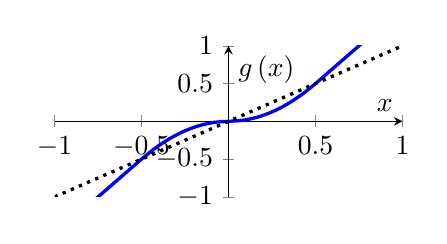
\begin{tikzpicture}[
      declare function={
        func(\x) = and(\x <= 0.5, \x >= 0) * (0.5*(abs(\x) / 0.5)^(2)) + 
        and(\x >= -0.5, \x < 0) * (-1*0.5*(abs(\x) / 0.5)^2) +
        (\x > 0.5)  * (2*(abs(\x) - 0.5) + 0.5) +
        (\x < -0.5) * ((-1)*(2*(abs(\x) - 0.5) + 0.5));
     } 
    ]
    \begin{axis} [
        axis lines=center,
	xmin=-1, xmax=1,
	ymin=-1, ymax=1,
        ylabel=\(g\left(x\right)\),
        xlabel=\(x\),
        width=6cm,
        height=3.5cm
      ]
      \addplot [domain=-1:1, smooth, very thick, blue] { func(x) };
      \addplot [domain=-1:1, smooth, dotted, very thick, black] { x };
    \end{axis}
  \end{tikzpicture}
  \caption{Response of the amplifier function \(g\) (\textcolor{blue}{blue line}) with \(\sigma=0.5\), \(\beta=2\).
  The dotted line shows a unity gain amplifier.}\label{fig:amp}
  %\vspace{-0.1in}
\end{figure}
%
The amplifier response curve is shown in~\cref{fig:amp}.
We can see that the low contrast values close to \(x=0\) are suppressed, and large contrasts are linearly amplified with a gain \(\beta=2\).

In the CLPD, we amplify the Laplacian image \({\boldsymbol\ell}_i\) using \(g\) before adding \(\widehat{\vg}_{i+1}\).
Therefore, both edges and noise are amplified before entering the filter \(F_i\), and the appropriate gain \(\beta\) thus depends on the characteristics of \(F_i\).

\subsubsection{Cascading Anisotropic Diffusion Filters}
For the filters \(F_0,\,\ldots\,, F_L\) used in the CLPD, we leverage anisotropic diffusion filters.
%Anisotropic diffusion equation-based filters are popular for enhancing the quality of medical ultrasound images~\cite{perona_scalespace_1990, weickert_anisotropic_1998, yongjianyu_speckle_2002, contrerasortiz_ultrasound_2012}.
These have shown strong speckle-noise reduction capabilities~\cite{duarte-salazar_speckle_2020}, strengthening of image edges~\cite{zhang_multiscale_2006}, and enhancement of image structures~\cite{abd-elmoniem_realtime_2002, kang_new_2016} with low computational cost (see~\cite{finn_echocardiographic_2011} for a comparative evaluation of some classic anisotropic diffusions).
However, they are also highly sensitive to their parameters~\cite{duarte-salazar_speckle_2020}, making them a perfect candidate for this study.

we follow the concept of~\cite{kang_new_2016} and use a different filter for each level.
We use the nonlinear coherent diffusion (NCD,~\cite{abd-elmoniem_realtime_2002}) and ramp-preserving nonlinear complex diffusion (RPNCD,~\cite{gilboa_image_2004}) filters.
Both NCD and RPNCD can be efficiently implemented on GPUs and have desirable properties for our purpose.
In comparison, recently introduced diffusion filters based on probabilistic tissue segmentation~\cite{vegas-sanchez-ferrero_probabilisticdriven_2010, ramos-llorden_anisotropic_2015} require accurately estimating a probabilistic mixture model during execution, which is computationally expensive and difficult to take advantage of GPUs.
Also, the recent method proposed by Mishra et al.~\cite{mishra_edge_2018} involves computing histogram of oriented gradients in the superpixel domain, which also cannot take advantage of GPUs.
%
\begin{figure}[t]
  \centering
  \subfloat[Original]{
    \includegraphics[trim={10cm, 10cm, 12cm, 5cm}, clip, scale=0.35]{figures/ncd_liver1.png}
  }
  \subfloat[NCD]{
    \includegraphics[trim={10cm, 10cm, 12cm, 5cm}, clip, scale=0.35]{figures/ncd_liver2.png}\label{fig:ncd}
  }
  \subfloat[RPNCD]{
    \includegraphics[trim={10cm, 10cm, 12cm, 5cm}, clip, scale=0.35]{figures/rpncd_liver.png}\label{fig:rpncd}
  }
  \caption{Example image processed with NCD and RPNCD.}\label{fig:ncd_liver}
  \vspace{-0.1in}
\end{figure}
%

Upper levels of the Laplacian pyramid contain image structures such as the myocardium in echocardiographic images or the portal veins in the liver.
In these levels, it is essential to recognize and enhance these structures.
Also, since upper levels focus on low frequencies, they contain less noise, allowing aggressive filtering.
For this, we leverage NCD, which is capable of enhancing spatial coherence~\cite{weickert_coherenceenhancing_1999}.
When naively applied to ultrasound images, coherence enhancement tends to interact badly with speckle noise, resulting in artistic flow-like artifacts as shown in~\cref{fig:ncd}.
In contrast, since the upper levels of the CLPD have less noise, NCD can aggressively enhance structures by coherence-enhancement.

On the other hand, lower levels contain lots of speckle noise and less structural information.
%Here, we shall use filters good at reducing speckle while preserving edges.
To perform speckle reduction, most anisotropic diffusion filters have to perform some sort of edge-detection.
This leaves us with a chicken-and-egg problem since the edge are obfuscated by speckle noise.
Meanwhile, diffusions based on Kuan and Lee's coefficients~\cite{yongjianyu_speckle_2002, aja-fernandez_estimation_2006, krissian_oriented_2007} do not perform explicit edge-detection but tend to result in blurry images.
To circumvent these issues, we propose to use RPNCD, which does not perform explicit edge-detection and does not rely on Kuan and Lee's coefficients.
RPNCD is based on a complex formulation of the anisotropic diffusion equation.
Gilboa \textit{et al.} showed that the phase evolution of the RPNCD acts like a smoothed Laplacian edge-detector, which is robust against noise.
We found that it shows excellent speckle reduction properties, as demonstrated in~\cref{fig:rpncd}.

The CLPD with edge-enhancement discussed in~\cref{section:edge_enhance} and the filters discussed in~\cref{section:edge_enhance} is shown in~\cref{fig:clpd}.
We use the NCD for the top two levels, while the RPNCD is used in the bottom.
Edge-enhancement is only performed on the bottom two levels.
We operate on log-compressed images where the pixels intensities are normalized to \([0, 1]\).
Specifically for the NCD, we rescale the input to \([0, 255]\) and the output back to \([0, 1]\).

\begin{table}
  \centering
  \caption{Parameters of the CLPD Tuned by the~\usdg}\label{table:params}
  \begin{threeparttable}
  \begin{tabular}{llrl}
    \toprule
    \multicolumn{1}{c}{\textbf{Parameter}}
    & \multicolumn{1}{c}{\textbf{Origin}}
    & \multicolumn{1}{c}{\textbf{Range}}
    & \multicolumn{1}{c}{\textbf{Scale}}
    \\ \midrule
    \(\sigma_{\mathrm{LL}_0}\), \(\sigma_{\mathrm{LL}_1}\)  & Edge-Enhance & [\(10^{\text{-}4}\), \(10^{\text{-}2}\)] & Exp.  \\
    \(\beta_{\mathrm{LL}_0}\), \(\sigma_{\mathrm{LL}_1}\)   & Edge-Enhance & [1, 5]                   & Lin. \\
    \(\alpha_{\mathrm{NCD}_1}\), \(\alpha_{\mathrm{NCD}_2}\) & NCD          & [\(0.03\), \(0.1\)]     & Lin.  \\
    \(s_{\mathrm{NCD}_1}\), \(s_{\mathrm{NCD}_2}\)           & NCD          & [\(1\), \(100\)]        & Lin. \\
    \(k_{\text{RPNCD}}\)                                & RPNCD        & [\(10^{\text{-}4}\), \(10^{\text{-}2}\)] & Exp. \\\bottomrule
  \end{tabular}
  \end{threeparttable}
  %\vspace{-0.1in}
\end{table}
%
%\vspace{-0.1in}
\subsubsection{Parameters of the Cascaded Laplacian Pyramid}
Our specific instance of the CLPD has 4 levels as shown in~\cref{fig:clpd}.
We use a decimation rate of 2 for all levels, while a pre-aliasing Gaussian low-pass filter (standard deviation 1) is applied before decimation.
The two edge-enhancement steps have two parameters each: the contrast threshold \(\sigma_{\mathrm{LL}}\) and the gain \(\beta_{\mathrm{LL}}\).
The unbiased NCD originally has 6 parameters: structure tensor smoothing rate\(\rho\), the step size \(\Delta t\), the number of iterations \(N_{\text{iter.}}\), the diffusion threshold \(s\), the diffusion strength coefficient \(\alpha\).
We set \(\rho = 2\), \(\Delta t = 2\), and \(N_{\text{iter.}} = 10\).
The other parameters are tuned by the~\usdg.
The RPNCD has 4 parameters: the edge threshold \(k\), the phase angle \(\theta\), the step size \(\Delta t\), and the number of iterations \(N_{\text{iter.}}\).
We set \(\theta = 5^{\circ}\) as proposed in~\cite{gilboa_image_2004}, \(\Delta t = 0.3\), and \(N_{\text{iter.}} = 20\).
The edge threshold \(k\) is tuned by the~\usdg.

While ideally, we would tune all the parameters using the~\usdg, BO takes longer to converge in high-dimensions.
Therefore, it is desirable to reduce the number of parameters as much as possible.
Also, nonlinearity between parameters makes the optimization problem fundamentally more challenging.
This happens when different parameters strongly depend on each other or have a similar effect.
For example, the effect of the diffusion step size \(\Delta t\) and iteration number \(N_{\text{iter.}}\) is determined by the product (diffusion time) \(\Delta t \cdot N_{\text{iter.}}\).
It is crucial to break up the nonlinearities by either leaving out some parameters or reparameterizing them.

The ranges and scales of the parameters to be tuned by the~\usdg~are organized in~\cref{table:params}.
A total of 9 parameters are tuned, resulting in a 9-dimensional optimization problem.
The number in the subscript denotes the level they are used within the pyramid (also refer to~\cref{fig:clpd}).
The range \([0, 1]\) used by the~\usdg~is transformed either linearly (Lin.) or exponentially (Exp.) to the range of the parameter.

%% \begin{align}
%%   \mT = K_{\rho} * \left( \nabla_{\sigma} I \; {\nabla_{\sigma} I}^{\top} \right) 
%% \end{align}
%% where \(K_{\rho}\) is a Gaussian smoothing filter with standard deviation \(\rho\), \(\nabla_{\sigma}I\) is the gradient of \(I\) smoothed with a Gaussian filter with standard deviation \(\sigma\).
%% NCD is known to 

%% Smoothing the outer product of the gradient with \(K_{\rho}\) improves the spatial coherence of the diffusion directions.
%% For the diffusion strengths \(\lambda_1\) and \(\lambda_2\), NCD uses the eigenvalues of the structure tensor \(\mu_1\) and \(\mu_2\) such that
%% \begin{align}
%%   \lambda_1 &= \begin{cases}
%%     \; \alpha \, \left(1 - \frac{\kappa}{s^2}\right) &  \text{if}\quad \kappa < s^2  \\
%%     \; 0 & \text{otherwise}\quad
%%     \end{cases} \\
%%   \lambda_2 &= \alpha
%% \end{align}
%% where \(\kappa = {(\mu_1 - \mu_2)}^2\), \(s\) is a threshold determining the amount smoothing towards \(\vv_1\), and \(\alpha\) determines the overall amount of smoothing.
%% While the original NCD algorithm uses a regularization term \(\beta\), we ommited it as we did not find it useful.

%% Meanwhile, Gilboa et al.~\cite{gilboa_image_2004} proposed a novel diffusion scheme that circumvents the need for explicit edge detection.
%% They proposed the \textit{ramp-preserving nonlinear complex diffusion} (RPNCD) which is described as
%% \begin{align}
%%   \frac{\partial  I\,(x, y, t)}{\partial t} &= \nabla \cdot \big(\, c\,(x, y, t) \, \nabla I(x, y, t) \big) \\
%%   c\left(x, y, t\right) &= \frac{e^{j \theta}}{ 1 + {\left( \frac{\mathrm{Im}\left(I(x, y, t)\right)}{ k \, \theta } \right)}^2}
%% \end{align}
%% where \(k\) is an edge threshold, \(\mathrm{Im}\left(I(x, y, t)\right)\) is the imaginary part of \(I(x,y,t)\), \(\theta\) is a phase angle parameter.
%% Here, \(\mathrm{Im}\left(I(x, y, t)\right)\) acts as an edge detector which behaves similarly as the smoothed image laplacian.


%% While many speckle reduction algorithms have been designed to be used on a single scale, many of these algorithms can be improved by considering \textit{multiple image scales}.
%% The two most popular approaches are based on the wavelet decomposition and the Laplacian pyramid decomposition.


%%% Local Variables:
%%% TeX-master: "master"
%%% End:
